\documentclass{beamer}

\usepackage[utf8]{inputenc}
\usepackage{amsmath,amsfonts,amssymb}
\usepackage{url}
\usepackage{listings}
\usepackage{color}
\usepackage{moresize}
\usepackage{algorithm}
\usepackage[noend]{algpseudocode}
\usepackage{graphicx} % Allows including images
\usepackage{booktabs} % Allows the use of \toprule, \midrule and \bottomrule in tables
\usepackage[style=numeric, backend=bibtex, maxcitenames=1, sorting=none]{biblatex}
\addbibresource{ipac21_sixtracklib.bib}


\definecolor{MyDarkMagenta}{rgb}{ 0.5, 0.0, 0.5 }
\definecolor{MyDarkBlue}{rgb}{ 0.0, 0.0, 0.5 }
\definecolor{MyDarkRed}{rgb}{ 0.5, 0.0, 0.0}
\definecolor{MyDarkOrange}{rgb}{0.667, 0.267, 0.0}
\definecolor{MyGray}{rgb}{0.6,0.6,0.6}

\let\oldfootnotesize\footnotesize
\renewcommand*{\footnotesize}{\oldfootnotesize\tiny}

\usetheme{Madrid}
\useinnertheme{circles}
\usecolortheme{dolphin}
\setbeamercovered{transparent}
\beamertemplatenavigationsymbolsempty
\usefonttheme{professionalfonts}

\title[SixTrackLib]{Optimising and Extending a Single-Particle Tracking Library for High Parallel Performance} % The short title appears at the bottom of every slide, the full title is only on the title page

\author[Schwinzerl et al]{M. Schwinzerl, R. De Maria, K. Paraschou, H. Bartosik, G. Iadarola, A. Oeftiger
\institute[CERN, GSI]{CERN, GSI} % Your institution as it will appear on the bottom of every slide,
}
\date{May 2021} % Date, can be changed to a custom date

% *************************************************************
% Bibliography
% *************************************************************

\setbeamertemplate{bibliography item}[text]

% *************************************************************

\begin{document}

\begin{frame}
\begin{figure}
 \centering
 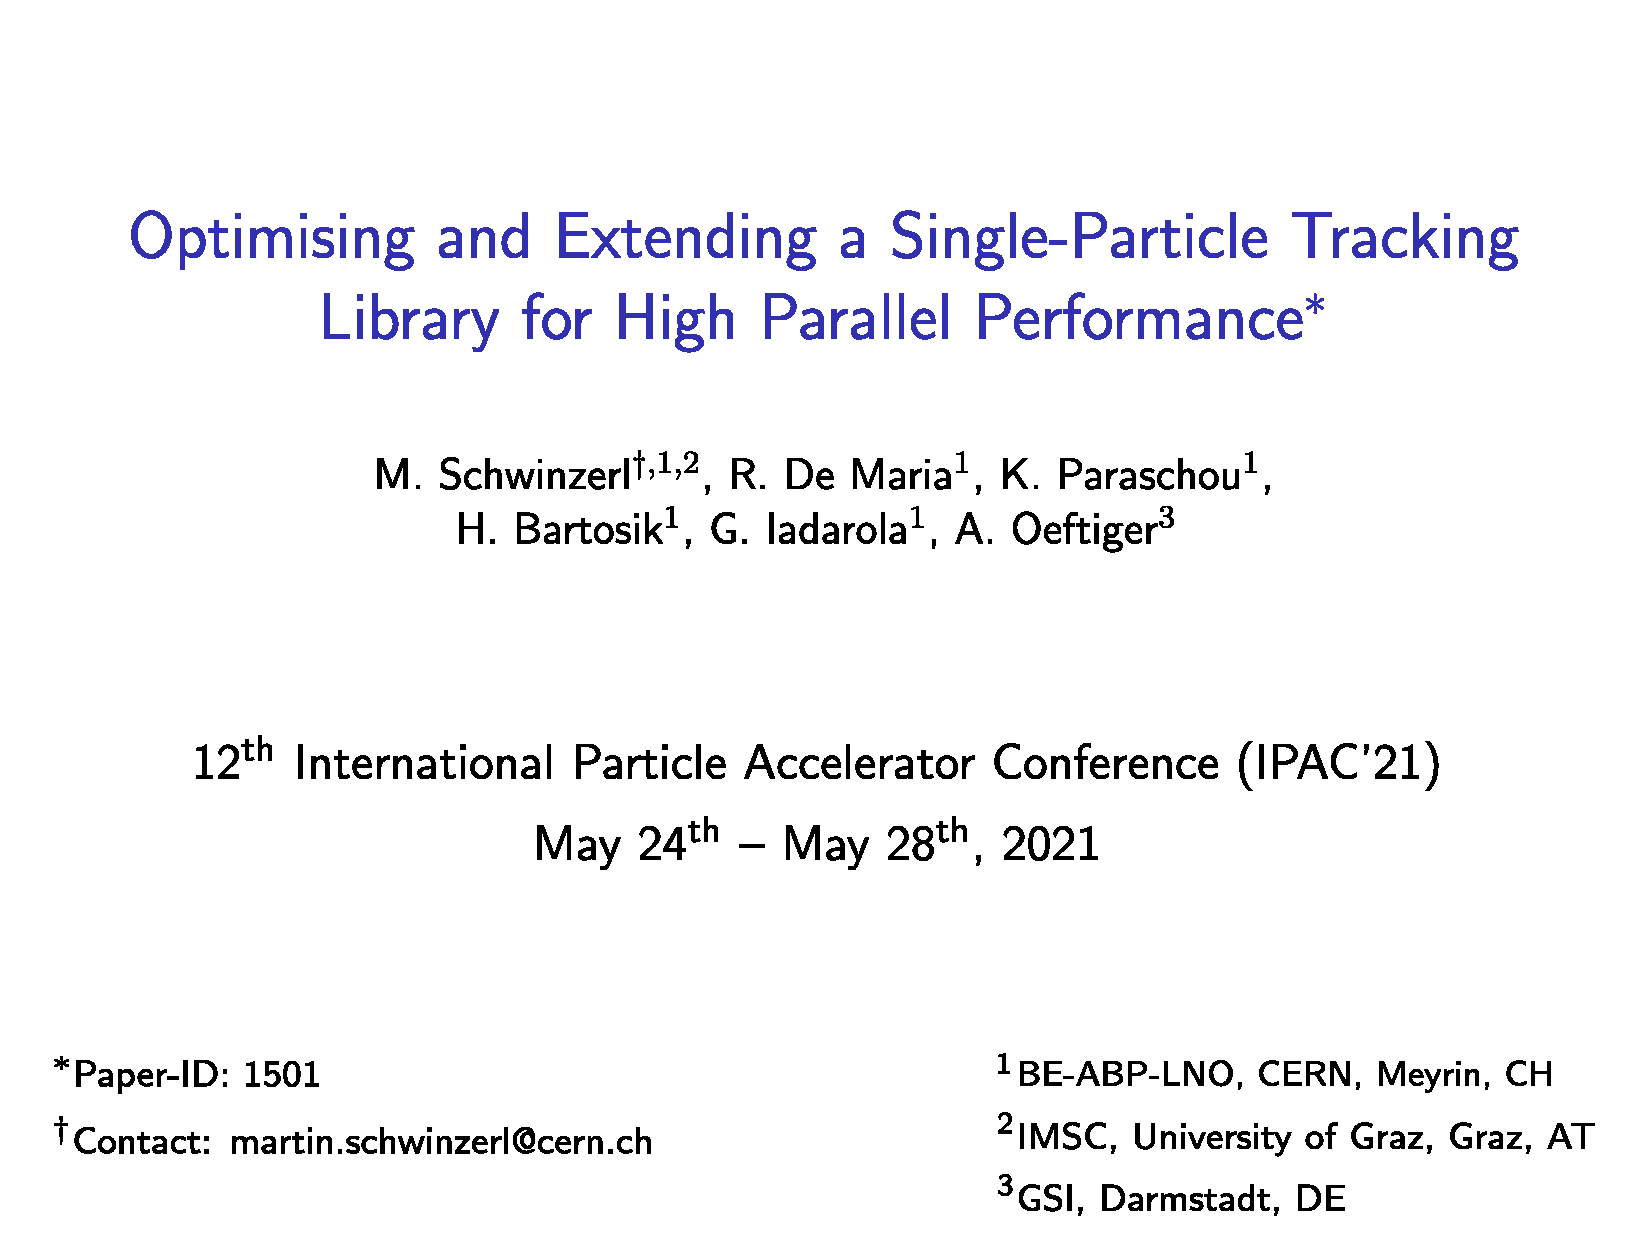
\includegraphics[width=0.95\textwidth]{poster_images/fig_title}
\end{figure}
\end{frame}

\begin{frame}[t]
\begin{abstract}
\texttt{SixTrackLib} is a library for performing tracking simulations on highly parallel systems such as shared memory multi-core processors or
graphical processing units (GPUs). Its single-particle approach fits very well to parallel implementations with reasonable base-line performance,
making such a library an interesting building block for various use cases, including simulations covering collective effects.\\[0.4em]

\noindent We describe the optimisations applied to \texttt{SixTrackLib} to improve its performance on its main target platforms and the associated performance gain.
Furthermore we outline the technical interfaces and extensions implemented to allow its use in a wider range of applications and studies.
\end{abstract}
\end{frame}

\begin{frame}
\frametitle{Outline}
\begin{itemize}
    \item Introduction
    \item Parallel Implementation
    \begin{itemize}
        \item Tracking Algorithm
        \item Baseline Parallel Implementation
        \item Feature Extensions \& Interfaces
    \end{itemize}
    \item Performance Analysis \& Optimisations
    \begin{itemize}
        \item Baseline Performance
        \item Optimisation Strategy
        \item Selected Results
    \end{itemize}
    \item Conclusions \& Outlook
\end{itemize}
\end{frame}

\begin{frame}
\frametitle{Introduction}
\begin{itemize}
    \item \texttt{SixTrackLib}\cite{sixtracklib-repo-2021} is a {\color{MyDarkBlue} single-particle} tracking library
    \item Re-implementation of the core \texttt{SixTrack}\cite{demaria-sixtrack-2019, sixtrack-repo-2021} tracking component
    \item Embeddable, minimal, usable on single CPU cores \& parallel hardware, multiple computing back-ends, common implementation of physics, high performance
\end{itemize}
\begin{figure}[h]
    \centering
    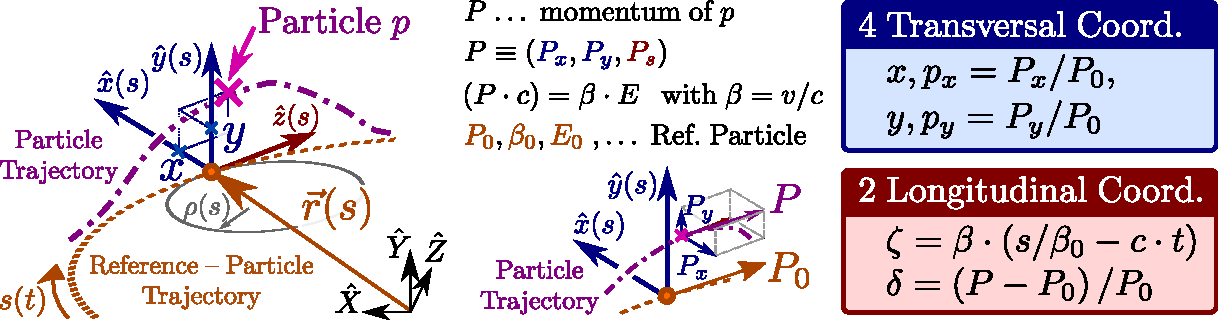
\includegraphics[width=0.95\textwidth]{poster_images/fig_coordinates_all}
\end{figure}
\begin{itemize}
    \item Particle $p \equiv p\left( x, p_x, y, p_y, \zeta, \delta\right)$ in $6D$ phase-space
    \item Coordinates expressed relative to a {\color{MyDarkOrange}Reference Particle}
\end{itemize}
\end{frame}

\begin{frame}
    \begin{center}
    {\HUGE\usebeamerfont*{frametitle}\usebeamercolor[fg]{frametitle}Implementation}
    \end{center}
\end{frame}

\begin{frame}[t]
\frametitle{Implementation - Tracking Algorithm}
\begin{itemize}
 \item Accelerator $\leadsto$ Sequence of idealised ``beam elements'' ({\color{MyDarkBlue}}Lattice)
 \item Map: describes the effect of a beam element $E_i$ on particle $p$
 \item Particles can get ``lost'' $\rightarrow$ stop tracking that particle
\end{itemize}

\begin{columns}
\begin{column}{0.6\textwidth}
\begin{algorithm}[H]
\small
\begin{algorithmic}
\Procedure{track\_until}{$\left(\mathbf{Q}\right)$, $\left(\mathbf{E}\right)$, $N$}
\For{$j \gets 1$ to $N_{p}$}\label{alg1:line:loop_particles}
    \State{ $p_j \equiv \left(\textbf{Q}\right)\left[j\right]$}\label{alg1:line:ref_p}
    \While{ $\left(
    \begin{array}{l}
        \mathbf{not} \; \texttt{is\_lost}(p_j) \; \mathbf{and} \\
                        \texttt{get\_at\_turn}(p_j) < N\\
    \end{array}
    \right)$}\label{alg1:line:loop_turns}
        \For{$i \gets 1$ to $N_{elem}$}\label{alg1:line:loop_lattice}
            \State{$E_i \equiv \left(\mathbf{E}\right)\left[i\right]$}\label{alg1:line:ref_elem}
            \State{$p_j \gets E_i\left( p_j\right )$}\label{alg1:line:apply_map}
            \If{$\texttt{is\_lost}(p_j)$}\label{alg1:line:is_lost_check}
                \State{ $\mathbf{break}$ }
            \EndIf
        \EndFor
        \If{$\mathbf{not} \; \texttt{is\_lost}(p_j)$}\label{alg1:line:is_lost_check2}
            \State $\texttt{increment\_at\_turn}(p_j)$\label{alg1:line:inc_turn}
        \EndIf
    \EndWhile
\EndFor
\EndProcedure
\end{algorithmic}
\end{algorithm}
\end{column}
\begin{column}{0.4\textwidth}
    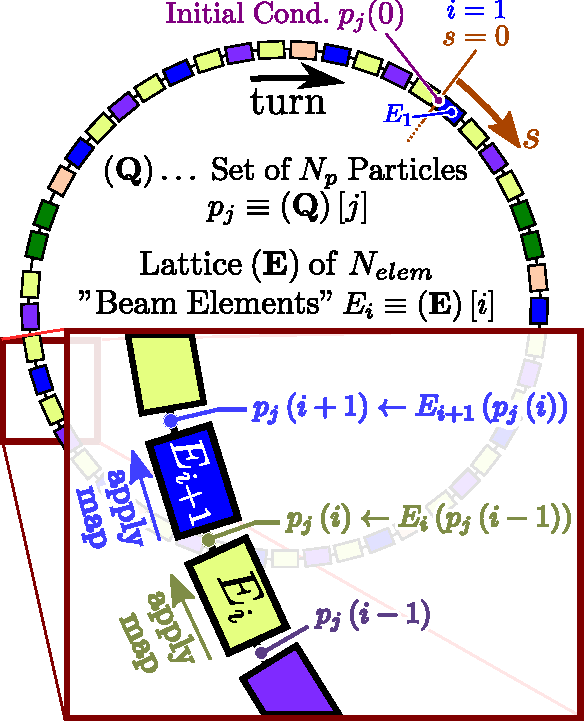
\includegraphics[width=0.9\textwidth]{poster_images/fig_tracking_algorithm}
\end{column}
\end{columns}
\end{frame}

\begin{frame}
\frametitle{Implementation - Baseline Parallel Implementation I}
\begin{itemize}
 \item Apply map $p_j\left(i+1\right) \gets E_i\left( p_j\left(i\right)\right)$: inherently sequential operation
 \item Only limited opportunity for parallelisation (e.g. \texttt{SIMD} vectorisation, \texttt{OpenMP} style loop-parallelisation, etc.) in specific maps $E_i$
 \item {\color{MyDarkBlue}Single-particle} tracking: $p_j$ and $p_k$ do not interact\newline
       $\Rightarrow$ For $N_p \gg 1$, the algorithm is embarrassingly parallel!
 \item Typical use cases $N_p = 1 \ldots >10^6$ particles, $N = 1 \ldots >10^7$ turns\newline
       $\Rightarrow$ Provide multiple {\color{MyDarkRed} computing back-ends}:\newline
       Vectorised for single-threaded CPU, \texttt{OpenCL 1.2}\cite{stone-opencl-2010}, and \texttt{CUDA}\cite{nickolls-cuda-2008}.
 \item Use {\color{MyDarkBlue} least common-denominator programming}:\newline
       Abstract differences between back-ends (\texttt{C99} kernel language, macros, grid conventions, etc.) $\rightarrow$ allows shared implementation of ``physics''.
 \item {\color{MyDarkRed}Required:} Common, efficient storage \& exchange container for structured data for all back-ends
\end{itemize}
\end{frame}

\begin{frame}
    \frametitle{Implementation - Baseline Parallel Implementation II}
    \begin{itemize}
        \item {\color{MyDarkBlue}Beam elements:} idealised, ``thin'', hard-edged, non-overlapping
        \item {\color{MyDarkBlue}Map:} Integrated solution to \emph{Hamiltonian Equations of Motion} $\rightarrow$ updates state of $p_{ii}$
        \item {\color{MyDarkRed}Example:} Map implementation for a {\color{MyDarkBlue}DriftExact} element:
    \end{itemize}
    \begin{figure}[H]
        \centering
        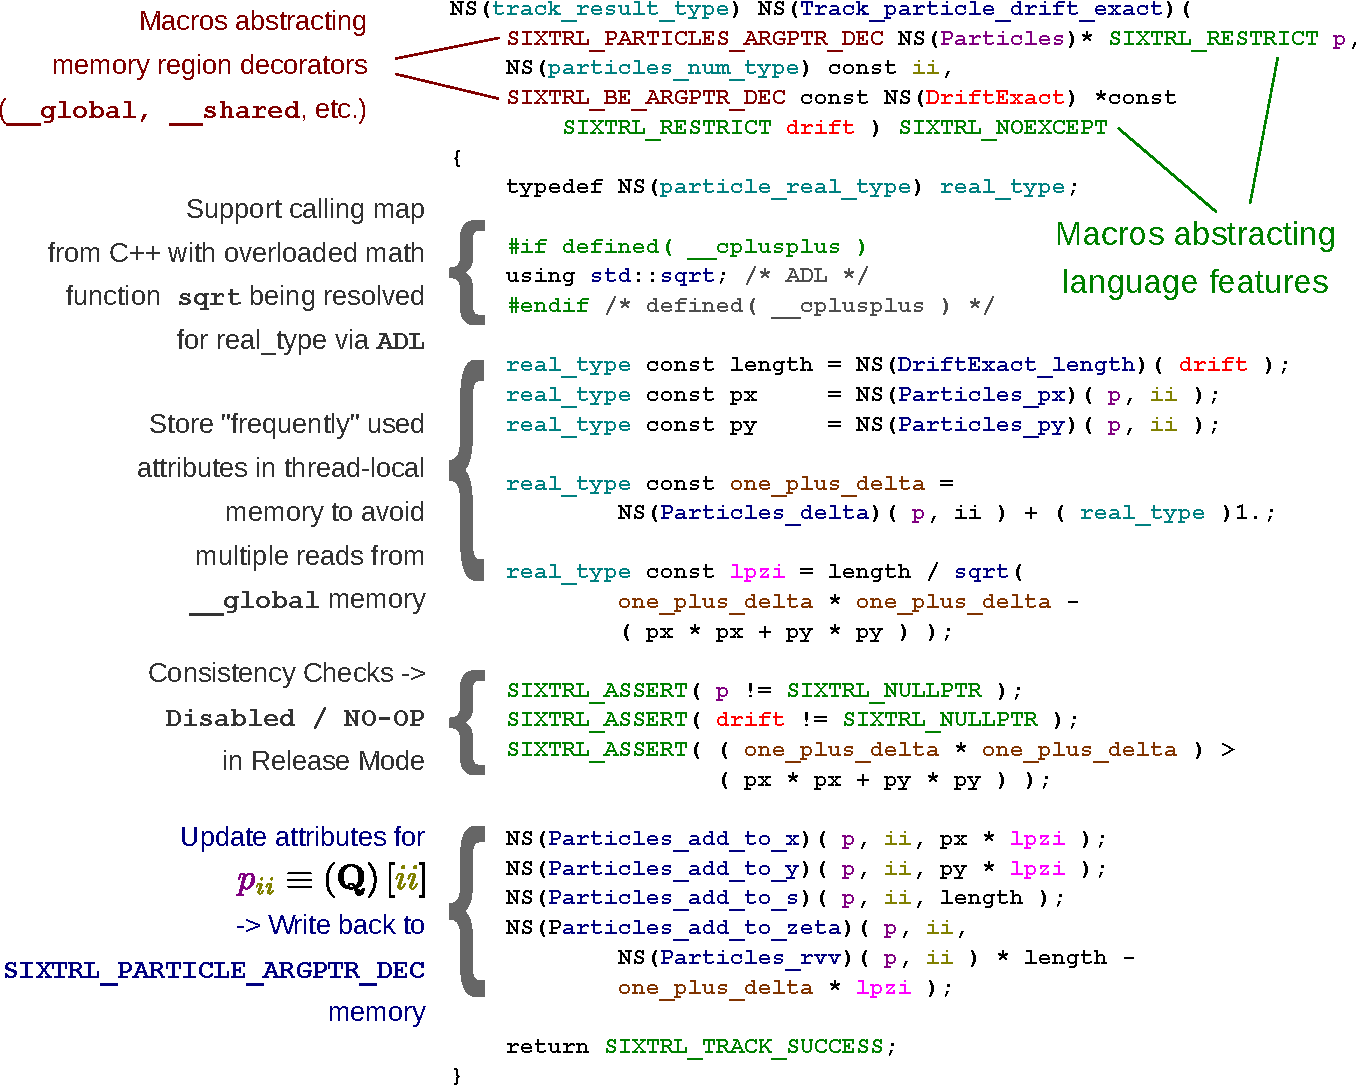
\includegraphics[width=0.6\textwidth]{poster_images/fig_map_drift_exact}
    \end{figure}
\end{frame}

\begin{frame}[t]
    \frametitle{Implementation - Baseline Parallel Implementation III}
    \begin{columns}
        \begin{column}{0.6\textwidth}
        \begin{itemize}
            \item Store {\color{MyDarkMagenta} sets of $N_p$ particles} $\left( \mathbf{Q} \right)$ in a \texttt{struct-of-arrays} fashion
            \item Replicate all attributes per particle:
            \begin{itemize}
                \item $6 \times$ \texttt{double} principle coordinates
                \item $5 \times$ \texttt{double} attributes of ref. particle
                \item $6 \times$ \texttt{double} auxiliary attributes to avoid re-calculation \& for convenience
                \item $4 \times$ \texttt{int64\_t} attributes for logistics
            \end{itemize}
            \item $\Rightarrow$ $21$ attributes \& $168$ Bytes of memory per particle
            \item Memory access can be coalesced, duplication of attributes (like for ref. particle) allows easier vectorisation
            \item {\color{MyDarkMagenta}Base-line implementation}: \texttt{global} memory (\texttt{OpenCL}, \texttt{CUDA})
        \end{itemize}
        \end{column}
        \begin{column}{0.4\textwidth}
            \begin{figure}[H]
                \centering
                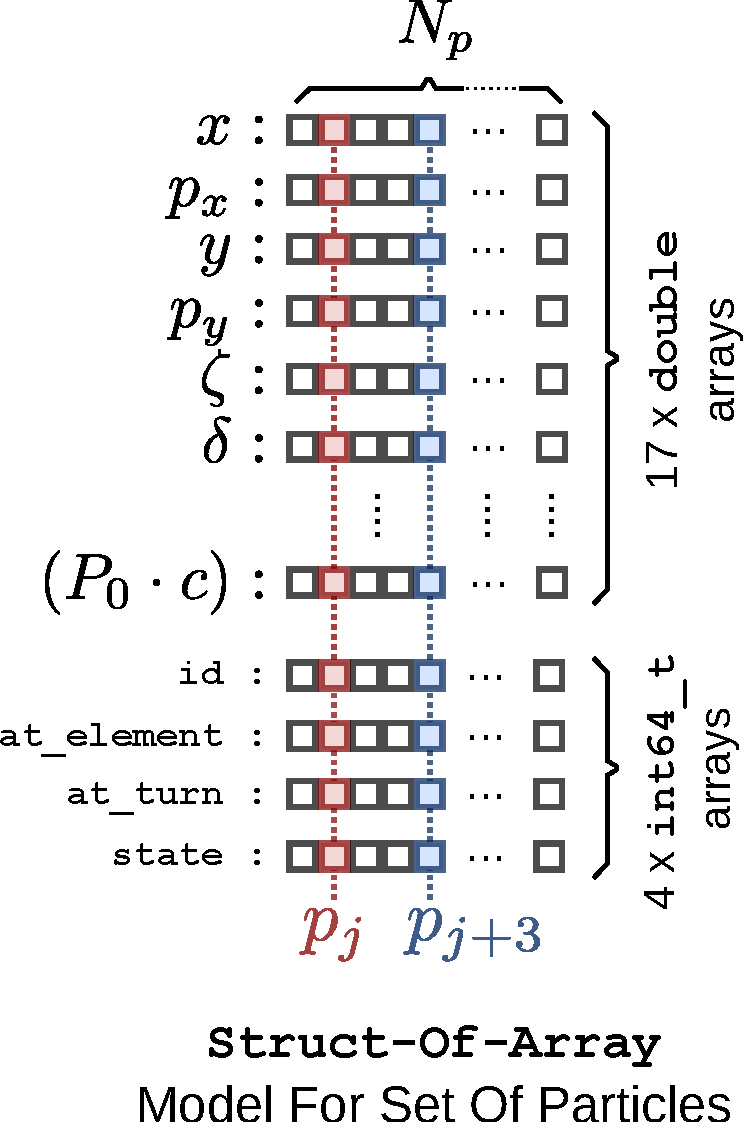
\includegraphics[width=0.95\textwidth]{poster_images/fig_particle_model_baseline}
            \end{figure}
        \end{column}
    \end{columns}
\end{frame}

\begin{frame}
    \frametitle{Implementation - Baseline Parallel Implementation IV}
    \begin{itemize}
        \item Storing \& exchanging buffers containing structured data with pointer data members is non-trivial.
        \item Copy: member pointers still point to initial location $\rightarrow$ \textit{re-mapping}
        \item \texttt{SixTrackLib} uses \texttt{cobjects}\cite{cobjects-repo-2021} buffers, allowing $\mathcal{O}(1)$
              lookup of stored elements, zero-overhead reading/updating of structured data
    \end{itemize}
    \begin{figure}[H]
        \centering
        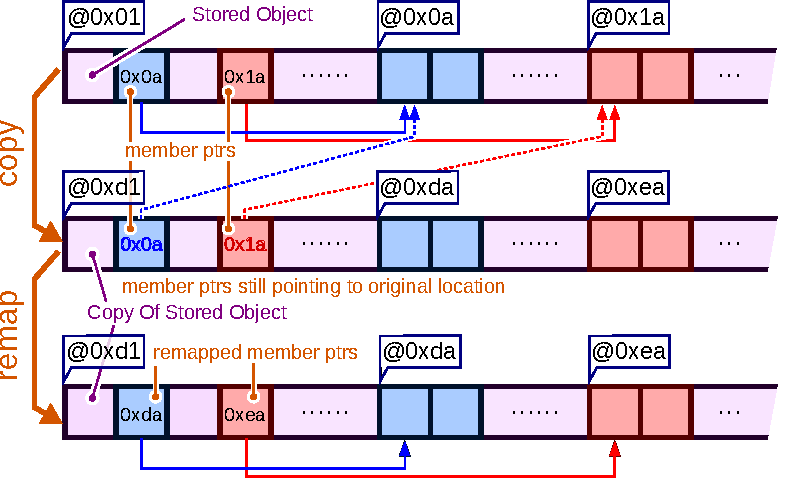
\includegraphics[width=0.5\textwidth]{poster_images/fig_cobjects}
    \end{figure}
    \begin{itemize}
        \item Drawback: more complicated to initially \textit{build} buffer with all stored elements, restrictions on alignment and complexity of structured data types
    \end{itemize}
\end{frame}

\begin{frame}
    \frametitle{Implementation - Extensions \& Interfaces I}
    \begin{itemize}
        \item \texttt{cobjects} allows excluding specific pointer members from remapping
        \item {\color{MyDarkBlue} Idea:} share data across multiple stored elements
        \item Challenge: manual remapping and assigning $\rightarrow$ \texttt{API} required
        \item {\color{MyDarkRed} Example:} Calculating symplectic kicks from electron cloud contributions via tri-cubic interpolation\cite{paraschou-iadarola-ecloud-2020}.
        Table with data $10^8$ to $10^9$ Bytes each $\rightarrow$
        has to be shared across lattice, otherwise too little memory even on high-end GPUs
    \end{itemize}
    \begin{figure}[H]
        \centering
        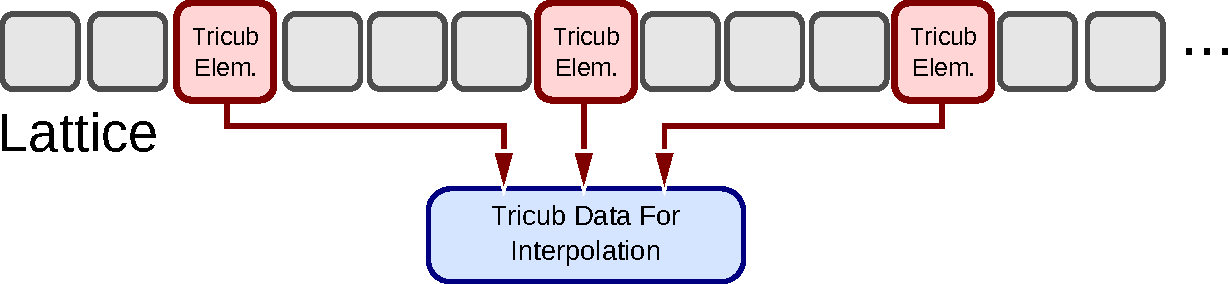
\includegraphics[width=0.8\textwidth]{poster_images/fig_be_external_data}
    \end{figure}
    \begin{itemize}
        \item {\color{MyDarkRed} Example:} Frozen space charge model with interpolated line charge density profile $\rightarrow$ discretised data is shared across space charge elements.
    \end{itemize}
\end{frame}

\begin{frame}
    \frametitle{Implementation - Extensions \& Interfaces II}
    \begin{itemize}
        \item \texttt{SixTrackLib}: lattice $\sim$ read-only, particles $\left( \mathbf{Q} \right)$ hold all state
        \item \texttt{PyHEADTAIL}\cite{pyheadtail-repo-2021} follows a similar approach
        \item {\color{MyDarkBlue}Idea:} Share particle state on GPUs (\texttt{CUDA}) and shared-memory CPUs (\texttt{OpenCL}) between \texttt{PyHEADTAIL} and \texttt{SixTrackLib}
        \item $\Rightarrow$ Hand-over tracking duties between \texttt{SixTrackLib} and \texttt{PyHEADTAIL} at specific points in the lattice\cite{oeftiger-spacecharge-2021}
    \end{itemize}
    \begin{figure}[H]
        \centering
        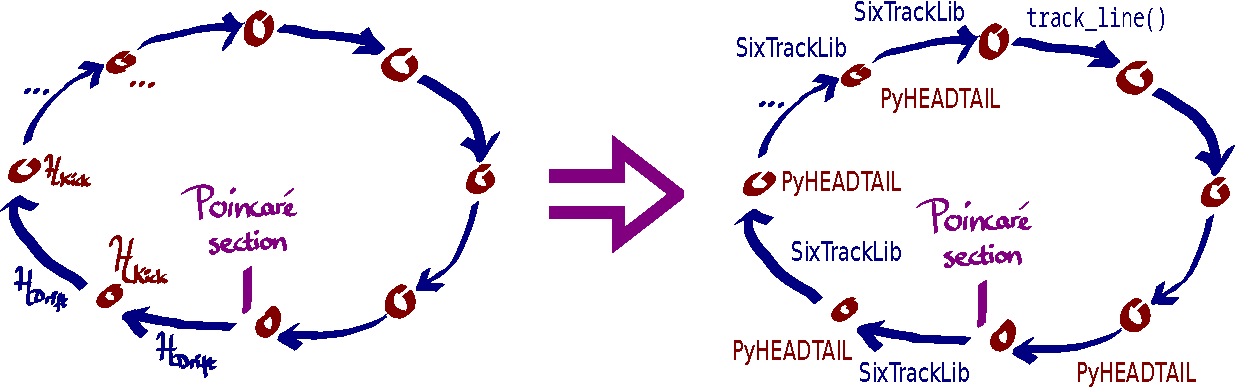
\includegraphics[width=0.7\textwidth]{poster_images/fig_pyheadtail_sixtracklib_integration}
    \end{figure}
    \begin{itemize}
        \item A modified version of the \texttt{track\_until} algorithm which only tracks a subset of the lattice in a single turn, \texttt{track\_line} is required
        \item Both this modification \& the sharing of data across stored beam elements limit and influence the applicability of some optimisations!
    \end{itemize}
\end{frame}

\begin{frame}
    \begin{center}
    {\HUGE\usebeamerfont*{frametitle}\usebeamercolor[fg]{frametitle}Performance Analysis \& Optimisation}
    \end{center}
\end{frame}

\begin{frame}
    \frametitle{Performance Analysis - Baseline Performance (Definitions)}
    \begin{itemize}
        \item The previously described implementation of \texttt{SixTrackLib} corresponds to \texttt{v0.5.0} on\cite{sixtracklib-repo-2021}
        \item {\color{MyDarkBlue}Lattice:} LHC with imperfections, without space charge or beam-beam interactions
        \item Vary $N_p$ from $10^0$ to $10^6$ particles, $(P_0 \cdot c) = 6.5\;\text{TeV}$, initial conditions so no particles are lost
        \item {\color{MyDarkBlue}Normalised tracking time:} $t_{track} = t_{elapsed} / \left( N_p \cdot N \right)$ (less is better)\newline
              $t_{elapsed}:$ elapsed wall-time, $N:$ number of turns
        \item Benchmark on a range of selected target systems\cite{data-repo-2021}:
        \begin{itemize}
            \item {\color{MyDarkRed}Single Core / Single Thread CPUs:} AMD Threadripper 2970wx and AMD Threadripper 1950x
            \item {\color{MyDarkRed}Multi-Threaded CPUs:} Same CPUs, but using the POCL and Intel OpenCL implementations, respectively
            \item {\color{MyDarkRed}Consumer-Grade GPUs:} NVIDIA GTX 1050 Ti and AMD Radeon VII
            \item {\color{MyDarkRed}HPC and High-End GPUs:} NVIDIA Titan-V and AMD MI50
        \end{itemize}
    \end{itemize}
\end{frame}

\begin{frame}
    \frametitle{Performance Analysis - Baseline Performance (Overview)}
    \begin{figure}[H]
        \centering
        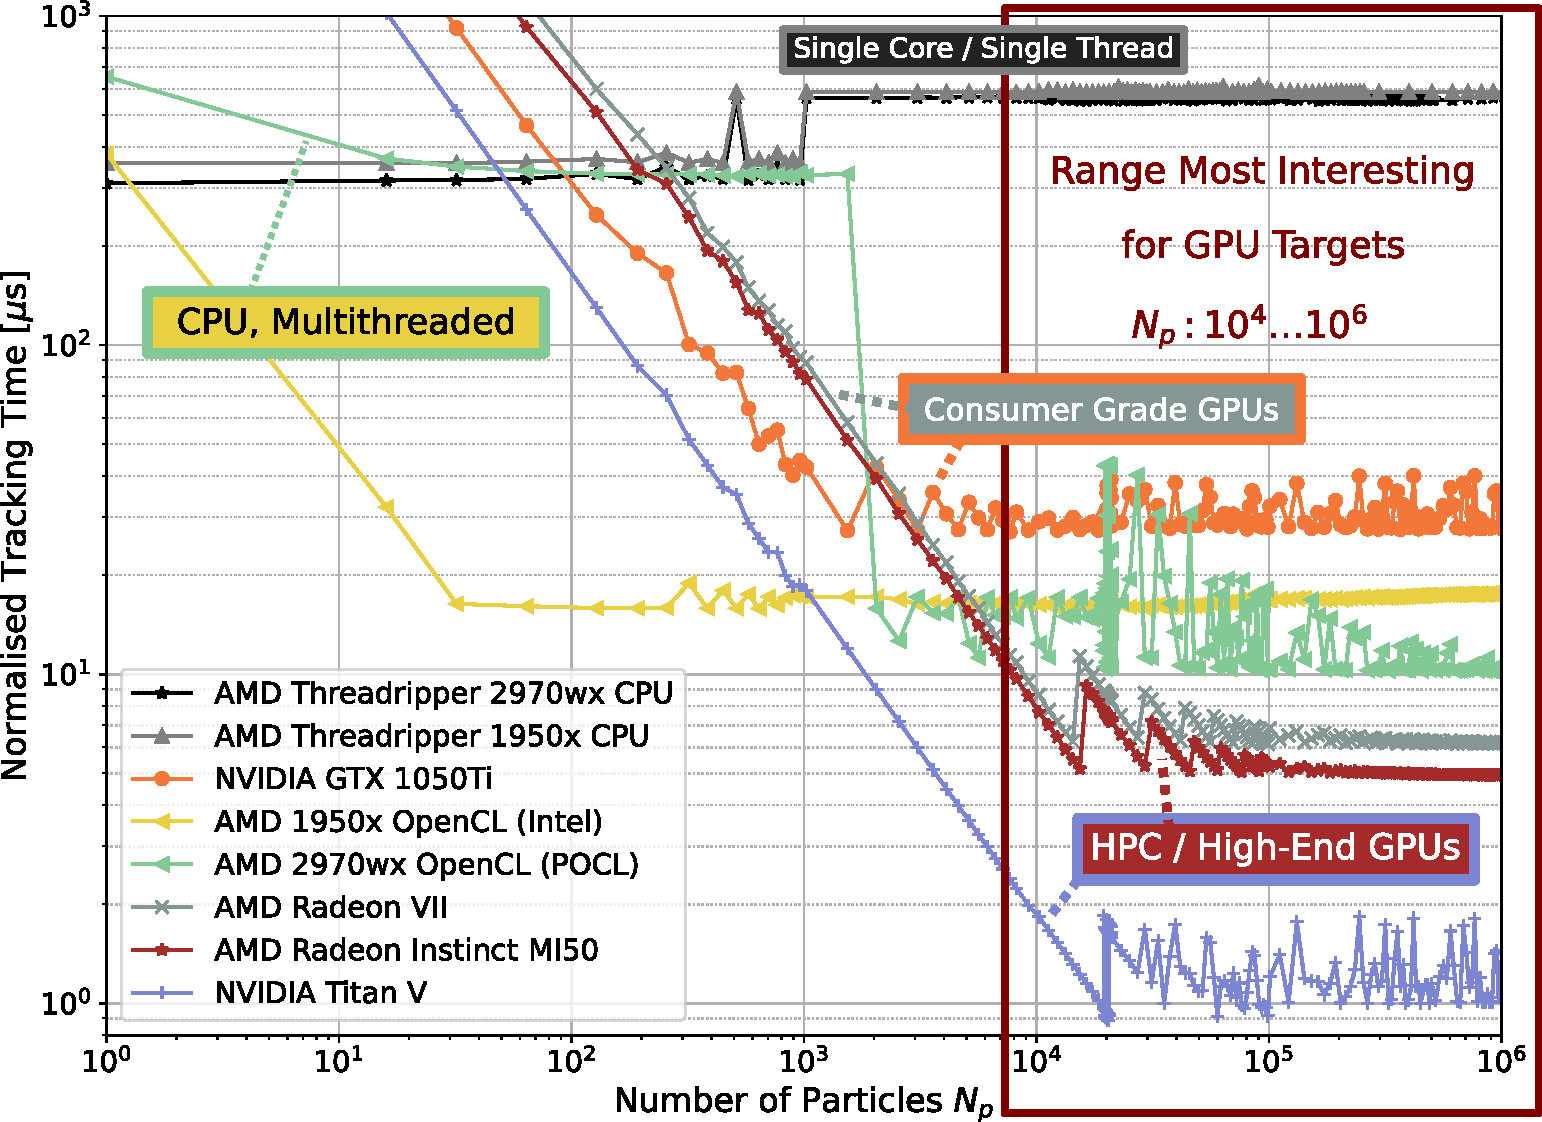
\includegraphics[width=0.75\textwidth]{poster_images/fig_benchmark_baseline_overview}
    \end{figure}
    \begin{itemize}
        \item {\color{MyDarkBlue}Expected:} $t_{track} \eqsim const.$ for single CPU and for $N_p$ large enough on parallel implementations (to compensate for overheads \& latencies)
    \end{itemize}
\end{frame}

\begin{frame}
    \frametitle{Performance Analysis - Baseline Performance (Detail)}
    \begin{itemize}
        \item $N_p = 10^4 \ldots 10^6$: all targets show expected behaviour
    \end{itemize}
    \begin{figure}[H]
        \centering
        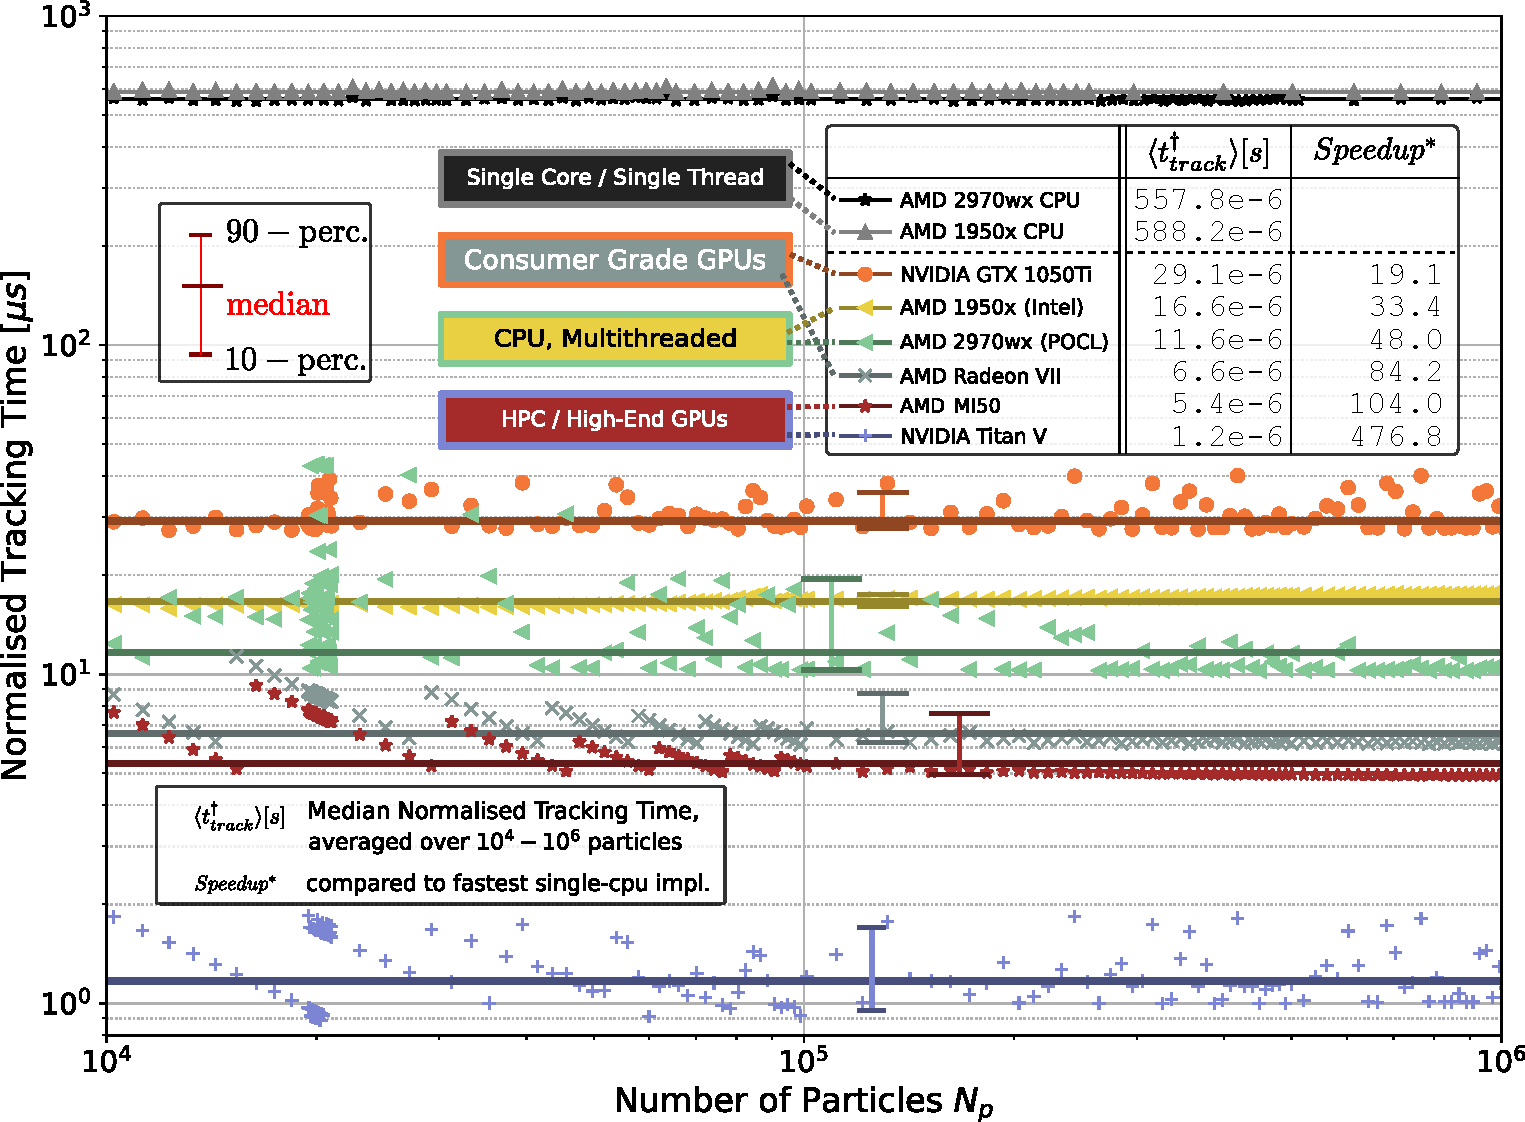
\includegraphics[width=0.75\textwidth]{poster_images/fig_benchmark_baseline_detail}
    \end{figure}
    \begin{itemize}
        \item Median parallel {\color{MyDarkBlue}speedups} range from $\mathcal{O}(10)$ to $\mathcal{O}(100)$
    \end{itemize}
\end{frame}

\begin{frame}
    \frametitle{Performance Analysis - Baseline Performance (Discussion)}
    \begin{itemize}
        \item All targets show expected behaviour for $N_p$ large enough to amortise overheads and latencies but variation in $t_{track}$ for similar $N_p$ $\Rightarrow$ use median $t_{track}$ to gauge avg. speedups
        \item For $N_p \eqsim 10^0$ to $10^1$, single CPU / single Thread implementations work best $\Rightarrow$ Sequential back-end is important!
        \item Single CPU performance is comparable to \texttt{SixTrack} and roughly maintains the performance level compared to recent \texttt{MAD-X}\cite{perssonMADXFutureColliders2021}
        \item For $N_p \eqsim 10^1$ to $10^3$, parallelisation on CPUs is typically more efficient than on most GPU systems
        \item Even consumer--grade GPUs with unfavourable \texttt{double} precision performance ratio (like $1:32$ for the GTX 1050 Ti) can reach
              $\mathcal{O}(10) \times$ better performance than the fastest studied single CPU system for large enough $N_p$
        \item High-end and dedicated HPC GPUs can attain speedups of $\mathcal{O}(100)$ for $N_p \geq 10^4$ particles
    \end{itemize}
\end{frame}

\begin{frame}
    \frametitle{Optimisations Strategies}
    {\usebeamerfont*{frametitle}\usebeamercolor[fg]{frametitle}a) Thread-Local Single-Particle Storage}\\[0.4em]
    \begin{figure}[H]
        \centering
        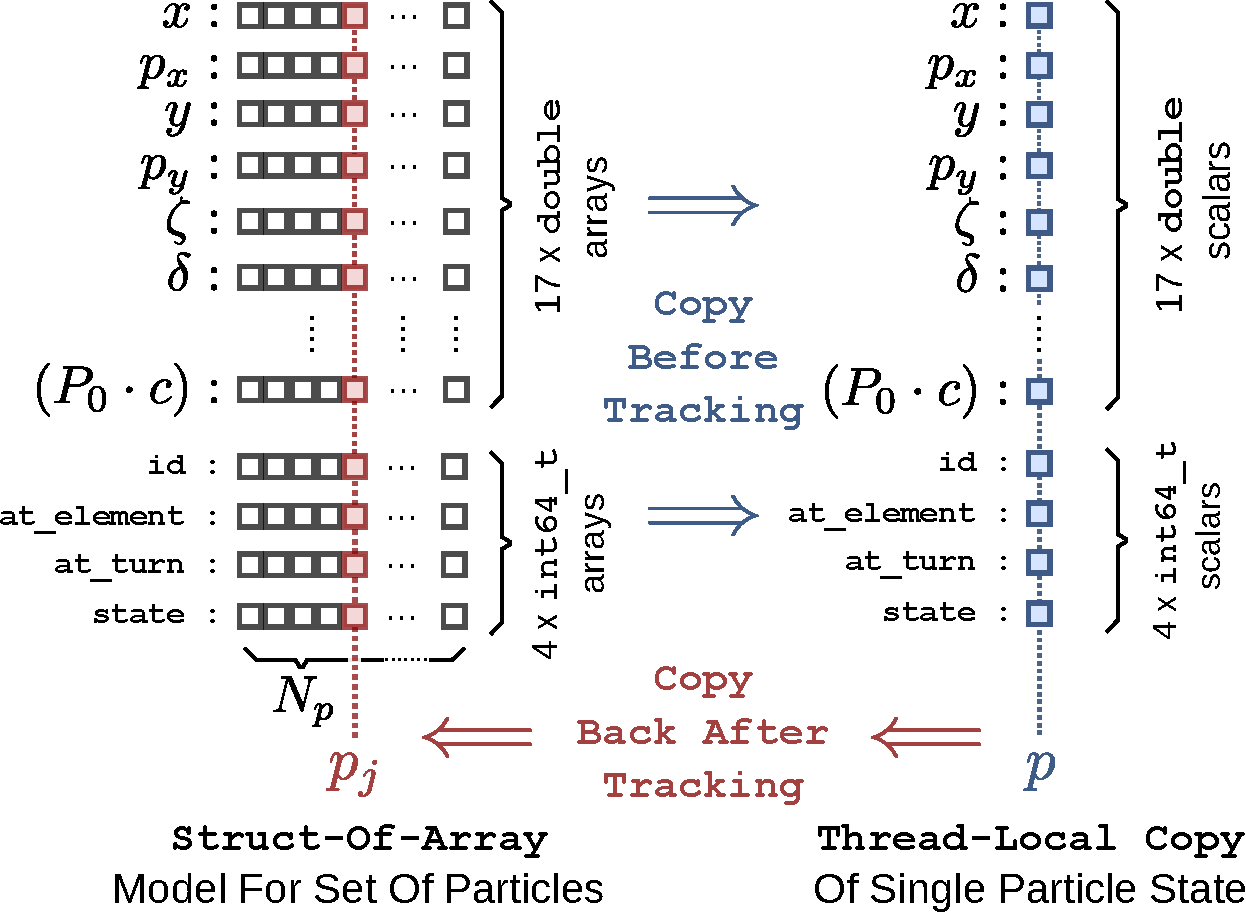
\includegraphics[width=0.5\textwidth]{poster_images/fig_particle_model_optimisation}
    \end{figure}
    \begin{itemize}
        \item Avoid global memory write-access for particle data $\Rightarrow$ provide each thread / work-item
           with a thread-local copy of $p_j$
        \item {\color{MyDarkRed}But:} increases register pressure $\Rightarrow$ Trade-offs especially if ``expensive'' maps are used (TriCubic interpolation, beam-beam interactions, etc.)
    \end{itemize}
\end{frame}

\begin{frame}
    \frametitle{Optimisations Strategies}
    {\usebeamerfont*{frametitle}\usebeamercolor[fg]{frametitle}b) Simplify Tracking Logic By End-Of-Turn Element}\\[0.4em]
    \begin{itemize}
        \item Nested loops in \texttt{track\_until} are difficult for compilers to optimise
        \item {\color{MyDarkBlue}Idea:} handle end-of-turn in map for dedicated beam element, always terminate lattices with such an element
    \end{itemize}
\begin{columns}
\begin{column}{0.6\textwidth}
\begin{algorithm}[H]
\small
\begin{algorithmic}
\Procedure{track\_until\_opt}{$\left(\mathbf{Q}\right)$, $\left(\mathbf{E}\right)$, $N$}
\For{$j \gets 1$ to $N_{p}$}
    \State{ $p \gets \left(\textbf{Q}\right)\left[j\right]\quad$ {\color{MyGray}{ /* Cf. a) */} }}
    \While{ $\left(
    \begin{array}{l}
        \mathbf{not} \; \texttt{is\_lost}(p) \; \mathbf{and} \\
                        \texttt{get\_at\_turn}(p) < N\\
    \end{array}
    \right)$}
        \State{$i \gets \texttt{get\_at\_element}( p )$}
        \State{$E_i \equiv \left(\mathbf{E}\right)\left[i\right]$}
        \State{$p \gets E_i\left( p\right )$}
        \State{\color{MyGray}/* increment of $\texttt{p.at\_element}$}
        \State{\color{MyGray}\hphantom{/* }performed while applying $E_i$ */}
    \EndWhile
    \State{$\left( Q \right)\left[ j \right] \gets p\quad$ {\color{MyGray}{ /* Cf. a) */} }}
\EndFor
\EndProcedure
\end{algorithmic}
\end{algorithm}
\end{column}
\begin{column}{0.4\textwidth}
    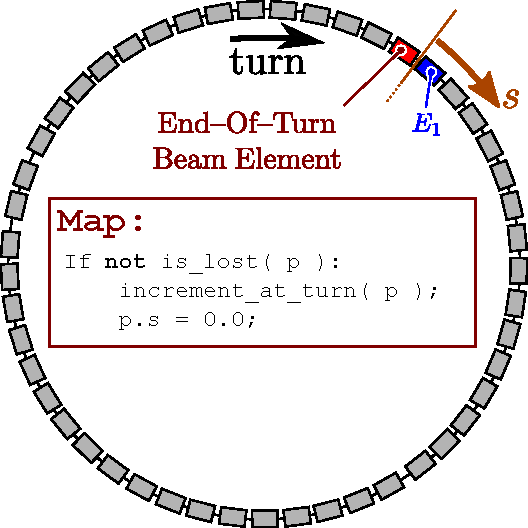
\includegraphics[width=0.9\textwidth]{poster_images/fig_tracking_algorithm_optimisation}
\end{column}
\end{columns}
\end{frame}

\begin{frame}
    \frametitle{Optimisations Strategies}
    {\usebeamerfont*{frametitle}\usebeamercolor[fg]{frametitle}c) Reduction Of Thread-Local Variables}\\[0.4em]
    \begin{itemize}
        \item Optimisations {\usebeamercolor*{frametitle} a) and b)} require changes to map $\Rightarrow$\newline
              Use $p$ being thread-local now to further eliminate variables storing intermediate calculations and cached expressions.
    \end{itemize}
    \begin{figure}[H]
        \centering
        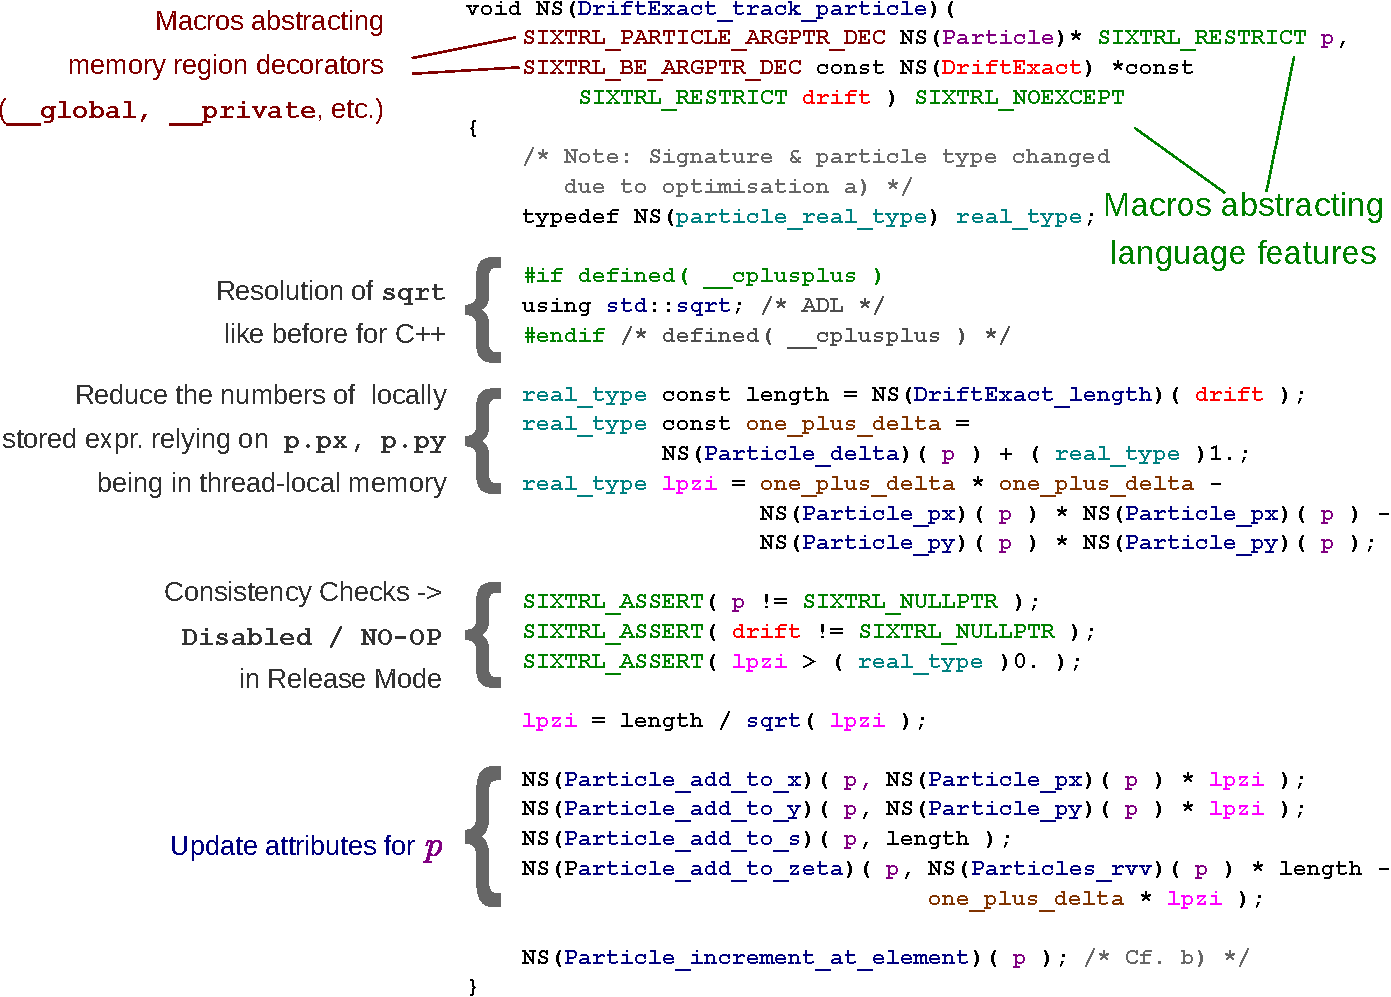
\includegraphics[width=0.6\textwidth]{poster_images/fig_map_drift_exact_optimisation}
    \end{figure}
\end{frame}

\begin{frame}
    \frametitle{Optimisations - Selected Results}
    \begin{itemize}
        \item Applying optimisations {\usebeamercolor*{frametitle} a), b), and c)} generally improves the run-time performance by a factor of $1.5$ to $2.0 \times$.
    \end{itemize}
    \begin{figure}[H]
        \centering
        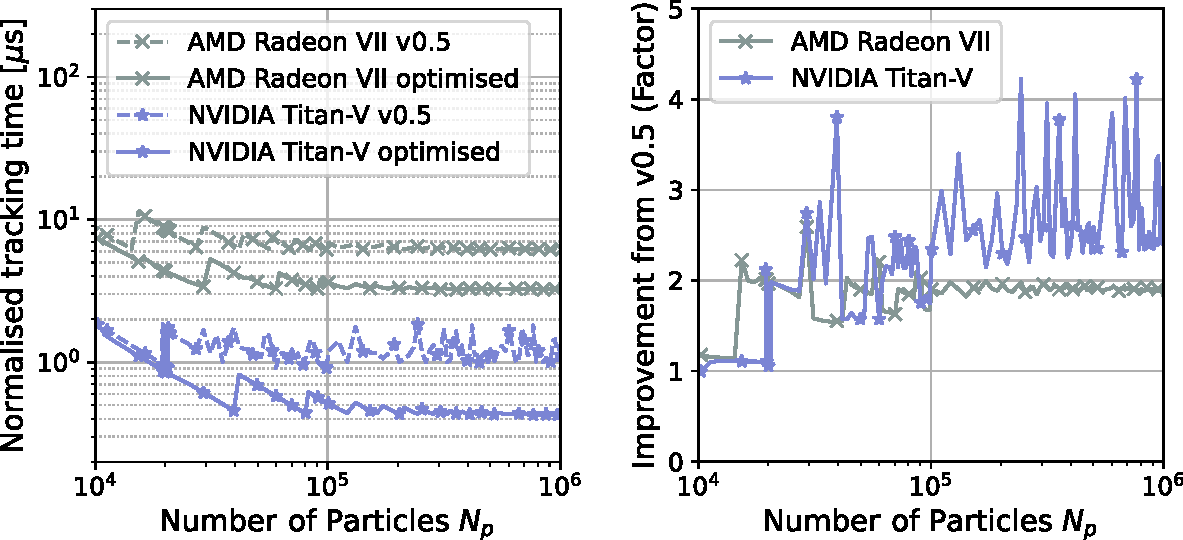
\includegraphics[width=0.9\textwidth]{poster_images/fig_performance_optimisation}
    \end{figure}
    \begin{itemize}
        \item For resource starved systems \& in the presence of maps inducing a high register pressure, the influence of especially {\usebeamercolor*{frametitle} a)} has to be carefully evaluated.
    \end{itemize}
\end{frame}

\begin{frame}
    \begin{center}
    {\HUGE\usebeamerfont*{frametitle}\usebeamercolor[fg]{frametitle}Outlook, Conclusions, References}
    \end{center}
\end{frame}

\begin{frame}
    \frametitle{Conclusions \& Outlook}
    \begin{itemize}
        \item Writing a tracking library with good parallel performance across a large range for $N_{p}$ \& for a diverse set of hardware is feasible.
        \item The presented (optimised) implementation performs satisfactory; sorted by increasing speedup, simulations profit from parallelisation on
        consumer-grade GPUs, multi-core high-end CPUs, and finally high-end and dedicated HPC GPUs.
        \item Further investigations about the contributing factors to the scaling behaviour are needed (esp. with respect to beam elements
              contributing significantly to the register pressure).
        \item If the extended interfaces and data sharing features are not needed, moving lattices to \texttt{constant} or \texttt{shared} memory could further improve performance.
        \item The presented optimisations will be part of the upcoming version 1.0 of \texttt{SixTrackLib}.
    \end{itemize}
\end{frame}


\begin{frame}[allowframebreaks, t]
    \frametitle{References}
    \tiny
    \printbibliography
\end{frame}
\end{document}
